%Created with command:
%"/home/josh/Teaching/trunk/Utilities/makeexam" "Homework 10 - Memory" "Please complete the problems below.  As usual you may work together.  However make sure the work that you submit is yours." "../Memory/Assessments/rom_name.tex" "../Memory/Assessments/ram_memory.tex"
\documentclass{article}
\usepackage[T1]{fontenc}
\usepackage{arev}
\usepackage{longtable}
\usepackage[hmargin=2cm,vmargin=2cm]{geometry}
\usepackage{graphicx}
\usepackage{listings}
\setlength{\parindent}{0pt}
\title{Homework 10 - Memory}
\date{}
\begin{document}
\maketitle
Please complete the problems below.  As usual you may work together.  However make sure the work that you submit is yours. (20 points total)
\begin{longtable}[l]{rp{17cm}}
%file: ../Memory/Assessments/rom_name.tex
1.&\begin{minipage}[t]{\linewidth}(10 pt) Design a ROM to store your first name using ASCII characters.  Address 0 of the ROM should output the ASCII code for the first character of your name, address 1 for the second character, etc.  Please specify how many address bits and data bits are required to store your name.\\ \\

Solution: \\ \\
The ASCII code for my first name is:\\
J $\rightarrow$ $0101010_2$\\
o $\rightarrow$ $1101111_2$\\
s $\rightarrow$ $1110011_2$\\
h $\rightarrow$ $1101000_2$\\ \\
This ROM uses 2 address bits and 7 data bits.\\ \\
\begin{center}
  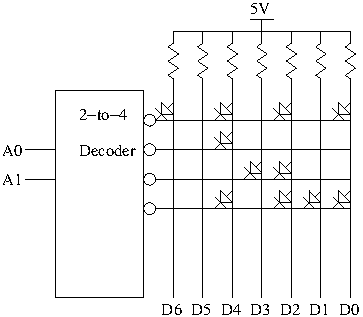
\includegraphics{../Memory/Assessments/ROMName}
\end{center}
\end{minipage}\\
\medskip
%file: ../Memory/Assessments/ram_memory.tex
2.&\begin{minipage}[t]{\linewidth}(10 pt) Design an SRAM with $n=4$ and $b=8$.  Use two 8x8 SRAM chips like the one we discussed in class to implement your SRAM.

Solution: \\ \\
\begin{center}
  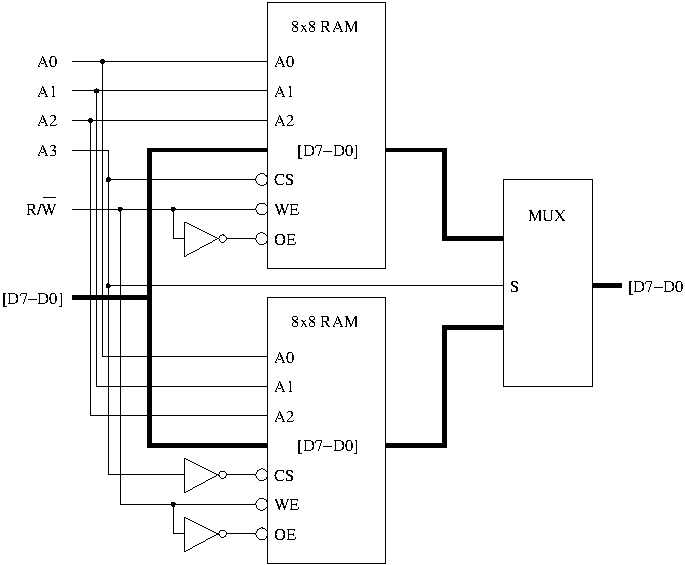
\includegraphics{../Memory/Assessments/RAMMemory}
\end{center}
\end{minipage}\\
\medskip
\end{longtable}
\end{document}